%\documentclass{article}
%\usepackage[pdftex,active,tightpage]{preview}
%\usepackage{tikz}
%\begin{document}
%\begin{preview}
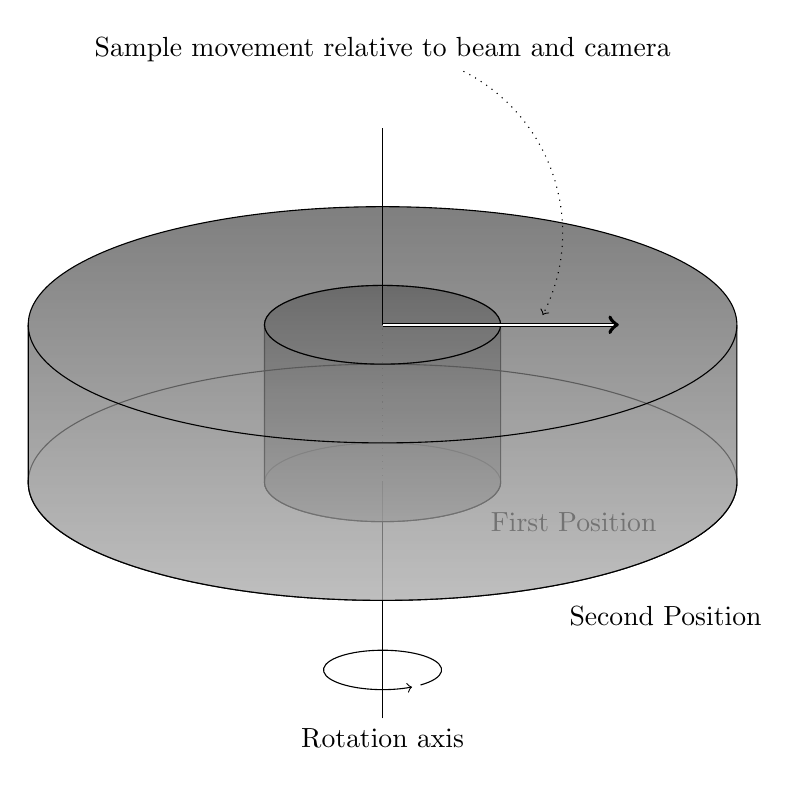
\begin{tikzpicture}%[ultra thick,scale=1]%,show background grid]
	%draw axes
		%\draw[ultra thick] (-10,0) -- (10,0);
		%\draw[ultra thick] (0,-10) -- (0,10);
		%\draw[ultra thick] (0,0) circle (.125);
	% rotation axis
		\draw[->] (0,-3) ++ (-50:.75) arc (-50:300:.75 and .25);
		\draw[] (0,-4) node [below] {Rotation axis} -- ++(0,3);
		\draw[dotted] (0,-1) -- ++(0,2);
	% position 1
		\draw (0,-1) circle (1.5 and .5);
		\fill[shade,semitransparent] (-1.5,-1) arc (-180:0:1.5 and .5) -- ++(0,2) arc (0:180:1.5 and .5) -- cycle;
		\draw (-1.5,-1) arc (-180:0:1.5 and .5) -- ++(0,2) arc (0:180:1.5 and .5) -- cycle;		
		\draw (-1.5,1) arc (-180:0:1.5 and .5);
		\draw (1.25,-1.5) node [right] {First Position};
	% position 2
		\draw (0,-1) circle (4.5 and 1.5);
		\fill[shade,semitransparent] (-4.5,-1) arc (-180:0:4.5 and 1.5) -- ++(0,2) arc (0:180:4.5 and 1.5) -- cycle;
		\draw (-4.5,-1) arc (-180:0:4.5 and 1.5) -- ++(0,2) arc (0:180:4.5 and 1.5) -- cycle;		
		\draw (-4.5,1) arc (-180:0:4.5 and 1.5);
		\draw (2.25,-2.7) node [right] {Second Position};
	% top from position 1 on top
		\draw (0,1) circle (1.5 and .5);
	% rotation axis on top
		\draw (0,1) -- ++(0,2.5);									
	% sample movement
		\draw[double,->] (0,1) -- (3,1);
		\node (movefrom) at (0,4.5) {Sample movement relative to beam and camera};
		\node (moveto) at (2,1) {};
		\draw [->,dotted] (movefrom) to [bend left=45] (moveto);
\end{tikzpicture}
%\end{preview}
%\end{document}